\documentclass[../../main.tex]{subfiles}
\begin{document}

\begin{problem}
\textbf{最大间隙问题}
一个 $2_k \times 2_k$ 个方格组成的棋盘中,恰有一个方格与他方格不同,称该方格为一特殊方格,且称该棋盘一特殊棋盘.
到棋盘覆盖问题囗棋盘覆盖问题是指,要用 4 种不同形态的 L 型骨牌覆盖给定的特殊棋盘上除特殊方格以外的所有方格,且任何 2 个 L 型骨牌不得重叠覆盖.
\end{problem}

\begin{solution}
    \begin{algorithm}[H]
        \caption{棋盘覆盖}
        \begin{algorithmic}[1]
            \Function{coverBoard}{$x, y, size, special\_x, special\_y$}
            \If{$size = 2$} \Comment{基本情况：处理 2x2 棋盘}
            \If{$special\_x = x \land special\_y = y$}
            \State 标记左上角为特殊方块
            \ElsIf{$special\_x = x \land special\_y = y+1$}
            \State 标记右上角为特殊方块
            \ElsIf{$special\_x = x+1 \land special\_y = y$}
            \State 标记左下角为特殊方块
            \Else
            \State 标记右下角为特殊方块
            \EndIf
            \State \textbf{return}
            \EndIf

            \State $half \gets size / 2$ \Comment{将棋盘分成四个子棋盘}
            \State 计算中心点 $(center\_x, center\_y)$

            \State 放置中心 L 型骨牌，使每个子棋盘有一个特殊方块
            \State \Call{coverBoard}{$x, y, half, \text{左上子棋盘特殊方块}$}
            \State \Call{coverBoard}{$x, y + half, half, \text{右上子棋盘特殊方块}$}
            \State \Call{coverBoard}{$x + half, y, half, \text{左下子棋盘特殊方块}$}
            \State \Call{coverBoard}{$x + half, y + half, half, \text{右下子棋盘特殊方块}$}
            \EndFunction
        \end{algorithmic}
    \end{algorithm}
    输入输出如下:
    \begin{figure}[htb]
        \centering
        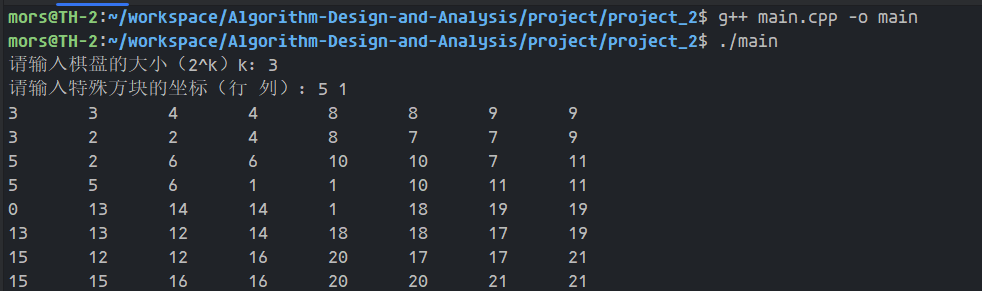
\includegraphics[width=450pt]{figure/Figure_1.png}
        \caption{输入输出示例}
    \end{figure}
    其中数字代表了L形骨牌的编号,编号从1开始,0代表特殊方格.
    \newpage
    该算法完整代码如下:
    \inputminted[
        frame=lines,
        framesep=2mm,
        baselinestretch=1.2,
        fontsize=\footnotesize
    ]{cpp}{project/project_2/src/main.cpp}


\end{solution}

\end{document}